%\chapter{det-comp}


%%%%%%%%%%%%%%%%%%%%%%%%%%%%%%%%%%%%%%%%%%%%%%
%\section{Anode Plane Assemblies}

%%%%%%%%%%%%%%%%%%%%%%%%%%%%%%%%%%%%%%%%%%%%%%
%\section{Cathode Plane Assemblies}

%%%%%%%%%%%%%%%%%%%%%%%%%%%%%%%%%%%%%%%%%%%%%%
%\section{Field Cage}

%%%%%%%%%%%%%%%%%%%%%%%%%%%%%%%%%%%%%%%%%%%%%%
%\section{HV components}

%%%%%%%%%%%%%%%%%%%%%%%%%%%%%%%%%%%%%%%%%%%%%%
%\section{TPC front-end electronics and DAQ}

%%%%%%%%%%%%%%%%%%%%%%%%%%%%%%%%%%%%%%%%%%%%%%
%\section{PDS front-end electronics and DAQ}

%%%%%%%%%%%%%%%%%%%%%%%%%%%%%%%%%%%%%%%%%%%%%%
%\section{Cryostat and feedthroughs}

%%%%%%%%%%%%%%%%%%%%%%%%%%%%%%%%%%%%%%%%%%%%%%  From David Montanari
\section{Cryogenics and LAr purification systems}
\label{sec:cryo-purif}

%%%%%%%%%%%%%%%%%%%%% 
\subsection{Overview, overall planning and ES\&H}

The scope of the ProtoDUNE Cryogenics includes the design, procurement, fabrication, testing, delivery, installation oversight and acceptance tests of a comprehensive cryogenic system that meets the performance requirements for purging, cooling down and filling the cryostat, acquiring and maintaining the LAr temperature within $\pm$1 K around nominal temperature (88.3 K), purifying the Liquid Argon (LAr) outside the cryostats, and re-condensing and purifying the boil-off Gaseous Argon (GAr).

The reference-design for the ProtoDUNE cryogenics infrastructure includes the External, Proximity and Internal Cryogenics.

%
The \textit{External Cryogenics} includes the systems used for the storage and eventual production of the cryogens needed for the operation of the cryogenic system (liquid ntrogen, LN2, for cooling; LAr for the cryostat) and GAr generated from the cryogenic storage tanks. In particular, it encompasses:
%
\begin{itemize}
\item The receiving facilities for LAr and LN2 tanker trucks;
\item The cryogenics transfer lines to deliver LAr and LN2 to the Proximity Cryogenics (in the vicinity of the cryostat);
\item The ambient vaporizer and transfer lines to deliver GAr to the cryostat for the piston purge and the GAr make-up; and
\item The regeneration system for the LAr purification (with GAr from the vaporizer and H2 from an H2 bottle, mixed before being sent to the LAr purification).
\end{itemize}
%
The \textit{Proximity Cryogenics} takes the cryogens from the External Cryogenics and delivers them to the Internal Cryogenics under the required pressure, temperature, purity and mass flow rate. It encompasses:
%
\begin{itemize}
\item The condenser (with heat exchanger) to re-condense the boil-off GAr;
\item The LAr purification system with inline purity monitor;
\item The LAr recirculation pumps;
\item The LAr Phase separator to feed the cryostat;
\item The LN2 Phase separator to feed the condenser;
\item The GAr purification system;
\item The cryostat-purge equipment; and
\item The condenser LAr pump.
\end{itemize}
%
The \textit{Internal Cryogenics} includes all the cryogenic equipment located inside the cryostat. It encompasses:
%
\begin{itemize}
\item The cryostat/detector cool down manifolds
\item The LAr distribution manifold
\item The GAr purge distribution manifold.
\end{itemize}
%
The equipment described in this chapter will be used for the cool-down, filling, operation, purification, emptying and warm-up of the ProtoDUNE Single Phase cryostat. These operations are described in greater detail in Section~\ref{sec:cryo-op-modes}.

The development of the ProtoDUNE cryogenics is part of a common effort between CERN and Fermilab which includes the cryogenics for the ProtoDUNE Single Phase and Dual Phase detectors at CERN, and the Short Baseline Neutrino Near Detector (SBND) and Far Detector (SBN-FD) at Fermilab.

The cryogenic systems for all four projects are developed jointly with a standard approach to minimize the duplication of work, benefit of existing knowledge (at Fermilab and CERN), and also prototype for the Long Baseline Neutrino Facility (LBNF)/Deep Underground Neutrino Experiment (DUNE) project. The systems build on the successful experience of the Liquid Argon Purity Demonstrator (LAPD), 35-t prototype, and MicroBooNE at Fermilab, and the development of the WA105 1$\times$1$\times$3 Dual Phase prototype at CERN and CERN's experience in the design and operation of large-volume noble liquid detectors.

%(FLC: I think not necessary here)The conceptual design for these cryogenic systems has been completed and an Invitation to Tender has been issued for the completion of the design, the fabrication, the delivery, the installation and the testing of all four systems, including the ProtoDUNE Single Phase detector. The replies to the tender have been received and CERN is negotiating with the potential suppliers, with the goal to award a contract after the CERN Finance Committee meeting scheduled for September. 

During all phases, CERN codes and standards will guide the design, procurement and installation phases of the ProtoDUNE Single Phase cryogenics. The planned work process provides for reviews throughout all phases of the project to guarantee stringent adherence to the safety and scientific requirements.

%%%%%%%%%%

%\subsubsection{Project requirements}  AH: I don't want to separate this into a subsubsection

%%%\fixme{ [Will this be written in another section?? If not, we can leave it here]DM}

The project requirements for the ProtoDUNE cryogenics system are identical to those of the DUNE Far Detector cryogenics. The current list 
of requirements is available at \cite{DUNE_FD_cryogenics_req}. 
%Note that the requirement numbers are subject to change.
%%% on DocDB n. 112 \fixme{Add citation}.

A selection of the most relevant requirements is presented here:
%
\begin{itemize}
\item Cryosys-013: The system shall allow recirculation and purification of the liquid argon inventory to achieve the needed LAr purity to meet the scientific requirement (less than 10 day/volume change based on ICARUS experience).
\item  Cryosys-016: The purification system shall be capable of removing contaminants form the LAr prior to filling and shall maintain purity during operation.
\item  FD-tpc-006: Electron lifetime greater than 3 ms (maximum drift time at nominal field is 2.25 ms).
\item  Cryosys-015: The system shall provide an argon gas boil off and reliquefaction system.
\item Cryosys-026: The cryogenics system shall not allow sources of argon gas reliquefaction inside the cryostat, e.g. uninsulated pipes carrying liquid argon.
\item  Cryosys-021: The cryostat and cryogenic systems shall be designed for using the piston-purge technique (introducing heavy gas at the bottom and taking out exhaust from the top) for removing initial electronegative impurities.
\item  Cryosys-019: The cryogenics system shall not introduce unwanted noise into the electronics.
\item  Cryosys-022: The cryogenics system shall provide a stable environment in the cryostat for the detector.
\item  Cryosys-023:The cryogenics system shall be designed in accordance with the cryostat to maintain a single phase in the entire liquid argon volume at a stable temperature. The chosen temperature is 88.3 K $\pm$ 1 K.
\end{itemize}

%%%%%%%%%%%%%%%%%%%%%

\subsection{Cryogenics layout}

The Process Flow Diagram (PFD) of the ProtoDUNE cryogenic system is shown in Figure~\ref{fig:cryo-process-flow}. The External Cryogenics located outside of the EHN1 building, is shared with the Dual Phase prototype, which is located in the same experimental hall, few tens of meters away.

\begin{cdrfigure}[Cryogenics process flow diagram]{cryo-process-flow}{Cryogenics process flow diagram} 
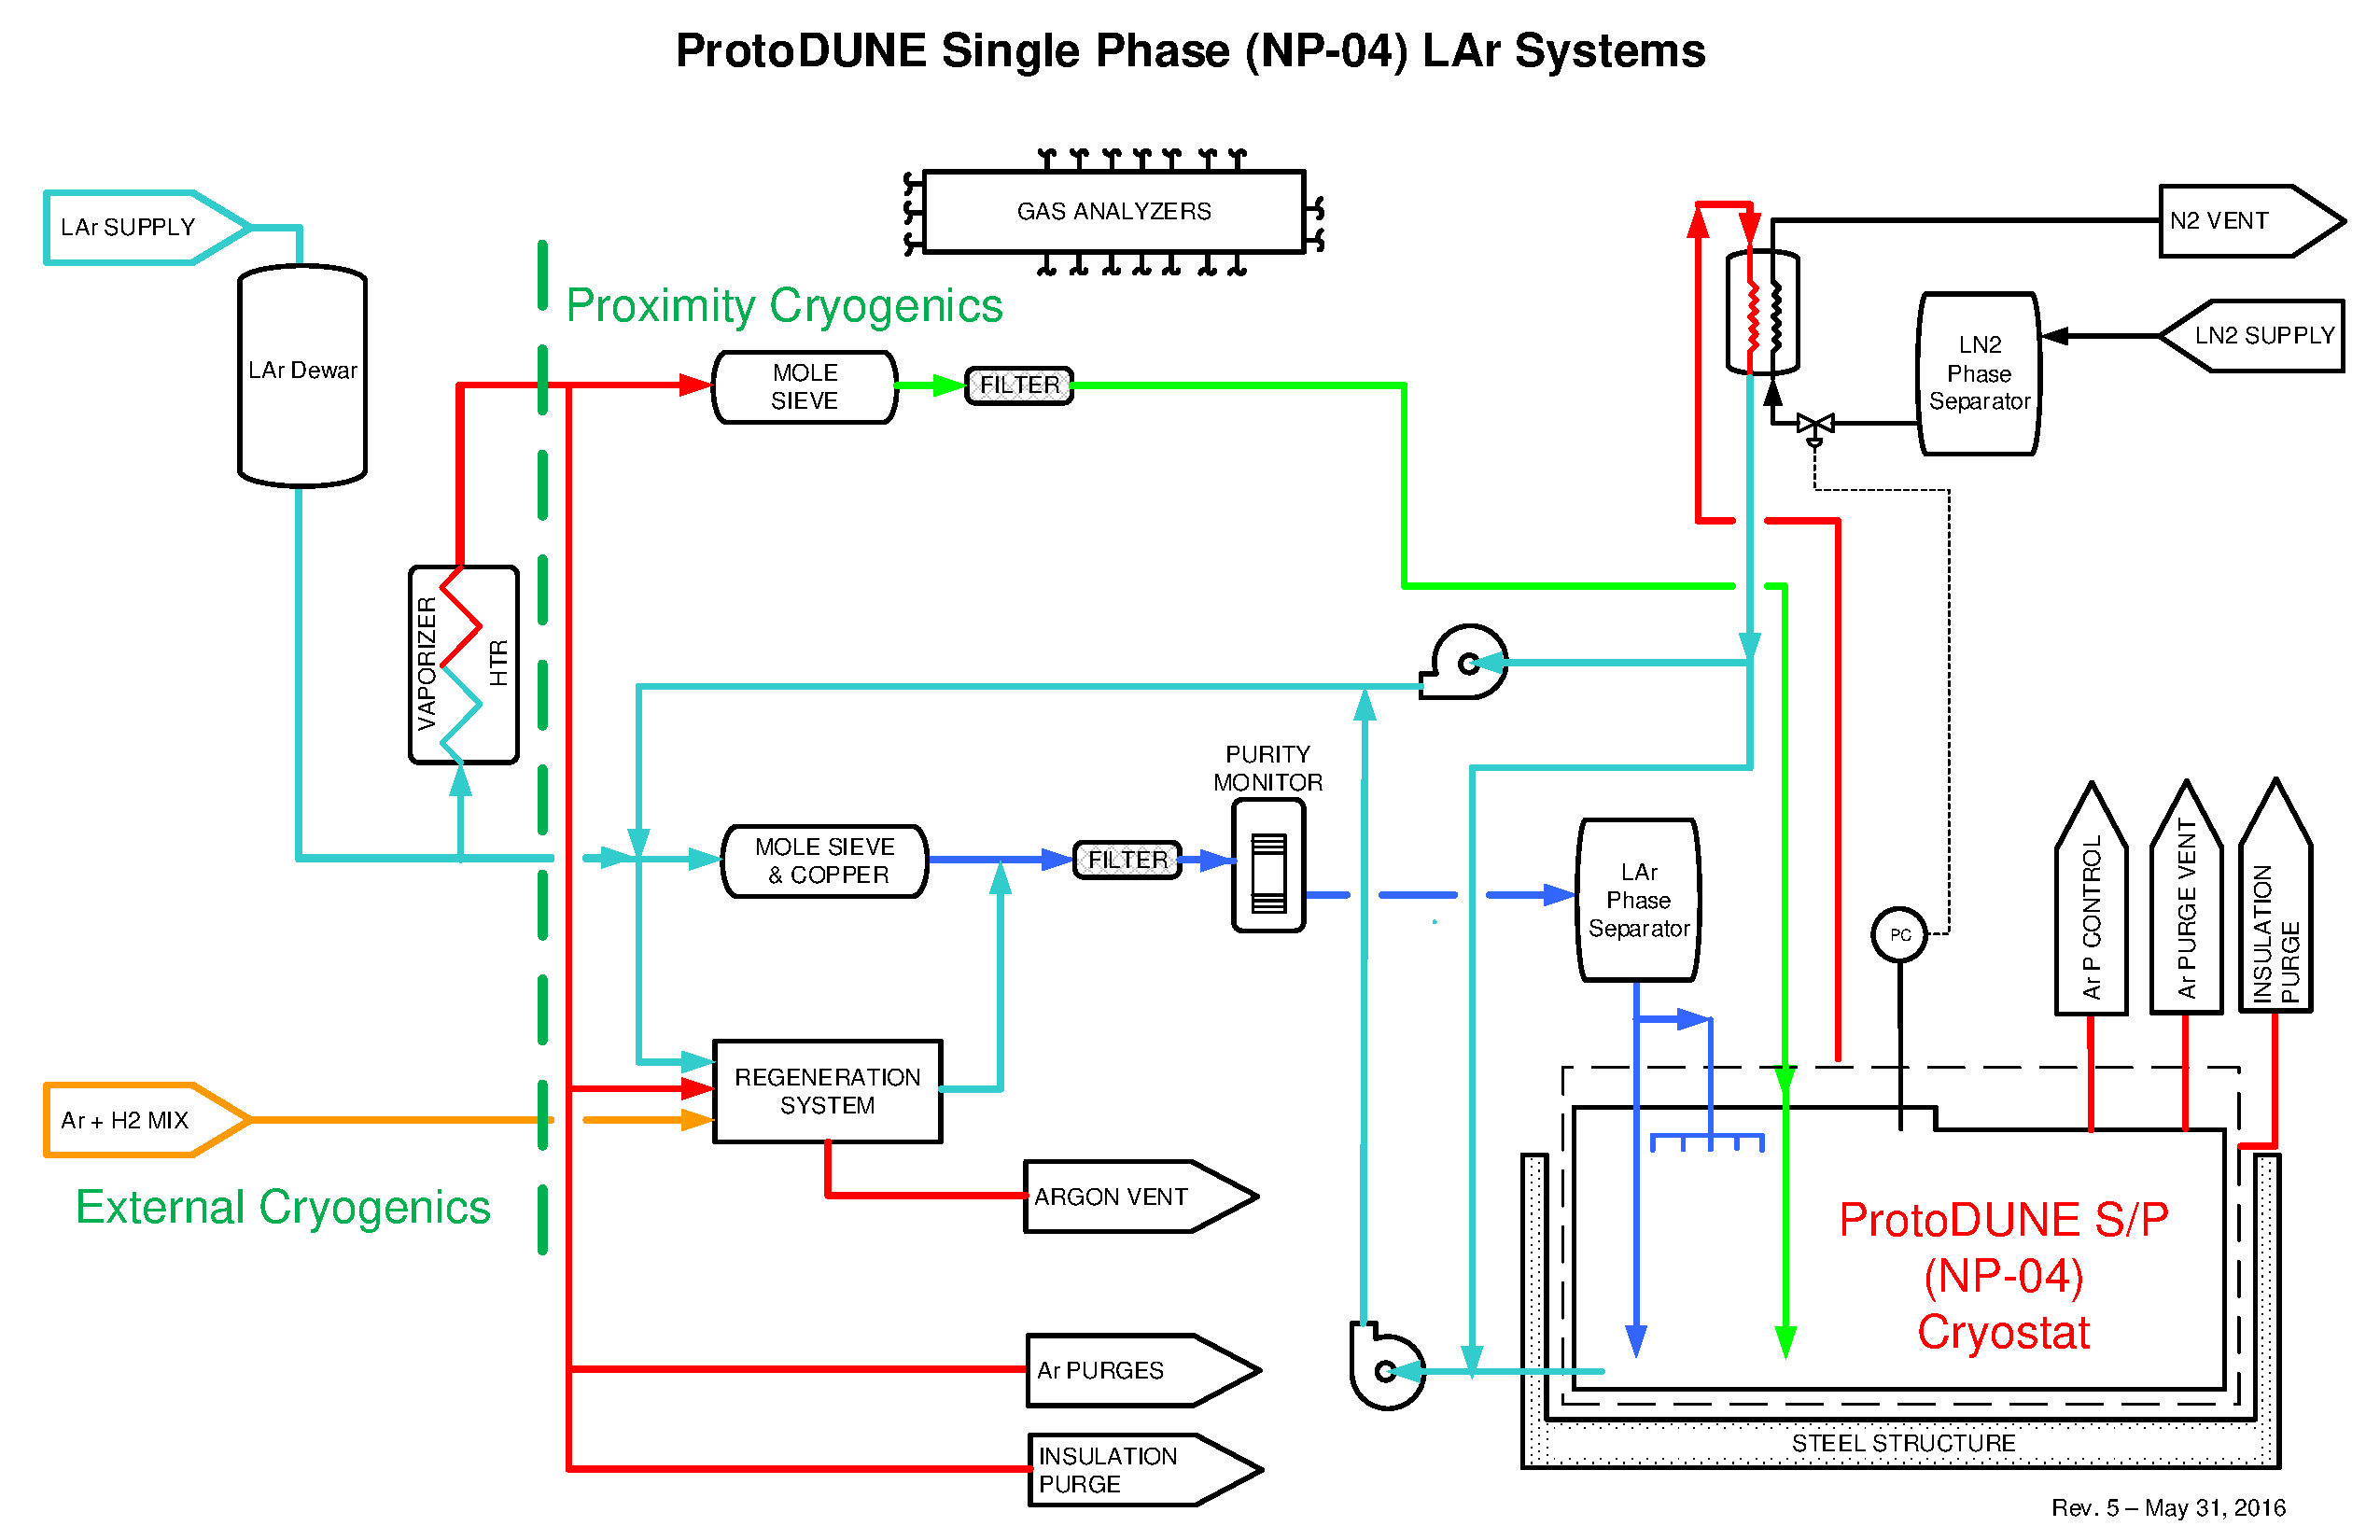
\includegraphics[width=0.95\linewidth]{cryo-process-flow}
\end{cdrfigure}

The system has the following functions:

\begin{itemize}
\item It provides the GAr for the piston purge phase and the GAr make-up.
\item  It provides the LAr to the cryostat.
\item  It provides the LN2 to the condenser.
\item  It provides the cooling power by means of evaporation of liquid nitrogen and condensation of GAr, to the liquid argon cryostat, for its cool-down, normal operation and warm-up phases.
\item  It provides the capability to purify the cryostat liquid argon volume to a level of parts per trillion (ppt) Oxygen equivalent contamination; the purification process uses mole-sieve and active copper.
\item  It provides the capability to purify the re-condensed boil off before reintroducing it inside the cryostat.
\item  It provides means to cool down the cryostat and the detector following the requirements.
\item  It distributes the LAr and GAr inside the cryostat to meet the requirements.
\end{itemize}

Figure~\ref{fig:3d-view-cryo-installation} shows a 3D view of the cryogenic installation as currently designed. The red and green lines entering  from the bottom of the figure are the LN2 and LAr supply lines, respectively, from the external cryogenics.
%
\begin{cdrfigure}[3D model of the installation ]{3d-view-cryo-installation}{3D model of the installation } 
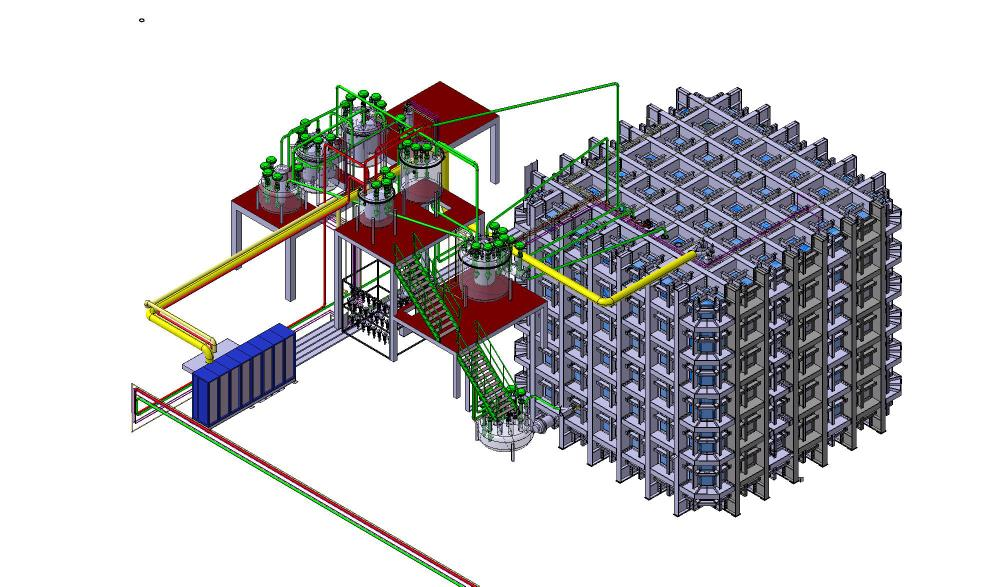
\includegraphics[width=0.85\linewidth]{3d-view-cryo-installation}
\end{cdrfigure}
%
Figure~\ref{fig:int-cryogenics-detail} shows a 3D view of a detail of the internal cryogenics: the cryostat and detector cool down manifolds at the top of the cryostat.
%
\begin{cdrfigure}[Detail of the internal cryogenics]{int-cryogenics-detail}{Detail of the internal cryogenics} 
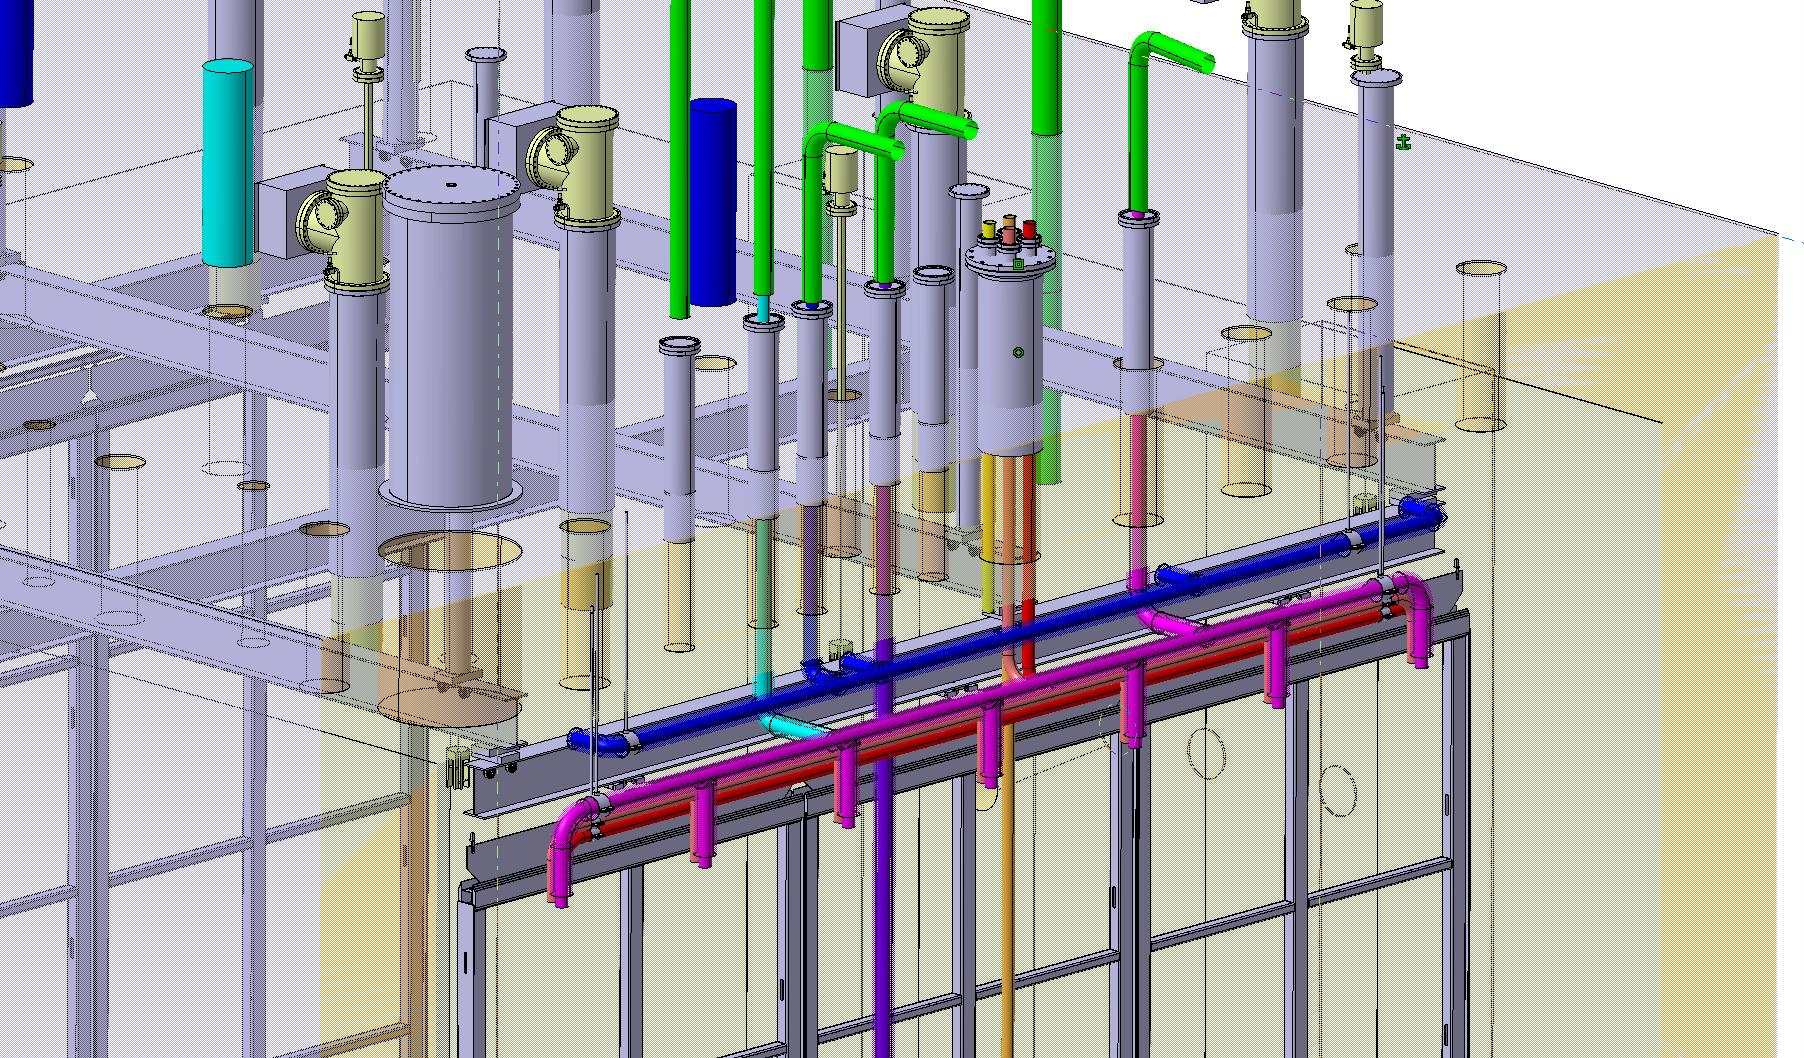
\includegraphics[width=0.9\linewidth]{int-cryogenics-detail}
\end{cdrfigure}

There is a common receiving facility for NP-02 and NP-04 located outside the building, from which Argon and Nitrogen lines take LAr, GAr, and LN2 to the respective installations.

A 50 m$^3$ (69 tons of LAr capacity) vertical dewar will allow for receipt of LAr deliveries for the initial filling period. This liquid argon dewar serves also as a buffer volume to accept liquid argon during the fill period. An analyzer rack with instruments to check water, nitrogen, and oxygen content of the delivered LAr batches will also be located in the vicinity. A 55-kW vaporizer is used to vaporize the liquid argon from the storage dewar prior to delivery to the GAr pipes.

The cryostat will have its own argon condenser (16 kW of cooling power), argon-purifying equipment and overpressure protection system. The full power of the argon condenser is used during the initial cool down phase only, which is expected to take two to three weeks. 

A 50 m$^3$ vertical dewar (40-t LN2 capacity) will allow for receipt of LN2 deliveries and storage of LN2 for cool down and normal operations. LN2 is flown into the heat exchanger of a condenser located in close proximity of the cryostat to recondense the boil-off GAr coming from the cryostat itself.

Two LAr recirculation pumps are placed outside of the membrane cryostat to circulate liquid from the bottom of the tank through the purifier and then back to the tank to ensure the needed LAr purity. 
%
The purification filters are located in the vicinity of the cryostat. The filters contain dual media, a molecular sieve for removal of water and a copper coated catalyst media for oxygen removal. There is one gas filter that is used during the purge in closed loop phase and two liquid filters used during the filling and normal operations to continuously purify the bulk of the LAr inside the cryostat. Associated with the filters, there will be regeneration equipment such as heaters, a GAr supply, a H2 bottle, and a way to mix GAr and H2. 
%
Before the Ar is returned to the cryostat, the LAr flows into a phase separator: the liquid is taken from the bottom and delivered to the cryostat, while the gas is returned to the condenser.


%%%%%%%%%%%%%%%%%%%%%
\subsection{Modes of operation}
\label{sec:cryo-op-modes}

The major functions of the cryogenics system servicing the cryostat are to supply cryogens for cool down and fill, and to provide gas argon filtration and condensing, liquid argon filtration and circulation. The methods presented in this section are motivated by experience from the cryogenic systems of other LAr Time Projection Chamber (TPC) experiments, such as ICARUS, LAPD, the 35 ton detector and MicroBooNE.

%%%%%%%%%%%%%%%%%%%%%
\paragraph{Cryostat piston purge}
%
After the cryostat construction and following the installation of all scientific equipment, the cryostat will be cleaned and purged in preparation for cool down and filling. Construction procedures leading up to this point will ensure that the completed cryostat does not contain debris and is free of all loose material that may contaminate the LAr.

%%%%%%%%%%%%
\paragraph{Purge in open loop}
%
Argon piping will be isolated, evacuated to less than 0.1 mbar  absolute pressure and backfilled with high-purity argon gas. This cycle will be repeated several times to reduce contamination levels in the piping to the ppm level. The reference-design choice for removing air from the membrane cryostat will be to flow/piston-purge argon, introducing the heavier argon gas at the bottom of the tank and removing the exhaust at the top. The exhaust will be taken from the main GAr outlet, but also from all the side ports located on each penetration through the roof to ensure that all volumes (especially trapped volumes) are properly purged.

The flow velocity of the advancing GAr will be set to 1.2 m/hour. This is twice the diffusion rate of the air downward into the advancing argon so that the advancing pure argon-gas wave front will displace the air rather than just dilute it. A 2D ANSYS model of the purge process shows that after about 13 hours of purge time and 2 volume changes, the air concentration will be reduced to less than 1\%. At 44 hours of elapsed time and seven volume changes, the purge process is complete with residual air reduced to a few ppm. This simulation includes a representation of the perforated field cage at the top and bottom of the detector and heat sources due to the readout electronics. %The cathode planes are modeled as non-porous plates although they will actually be constructed of stainless-steel mesh. 

The Computational Fluid Dynamics (CFD) model of the purge process has been verified in multiple arrangements: (1) in an instrumented 1 m-diameter by 2 m-tall cylinder, (2) in LAPD, a 3 m- diameter by 3 m-tall cylindrical tank where gas-sampling measurements were at varying heights and times during the purge process, and (3) within the 35 ton membrane cryostat, the prototype vessel built at FNAL in 2013. The results of these tests are available in~\cite{lar1-nd-35-ton-talk} and~\cite{CFD_verification-lapd}. 
%
Once the residual air inside the tank is at the the ppm level, the process continues in the closed loop configuration. 

%%%%%%%%%%%%
\paragraph{Purge in closed loop}

Water and oxygen will continue to be removed from the system for several days following the initial purge. During this step the GAr is no longer exhausted but recirculated through the GAr purifier and sent back to the bottom of the cryostat. The cryostat contains a relatively large amount of FR4 circuit-board material and a smaller inventory of plastic-jacketed power and signal cables. These somewhat porous materials may contain as much as 0.5\% water by weight. Water-vapor outgassing from these materials will be entrained in the gas flow exiting the top of the cryostat and will be removed from the gas stream by filters. Adsorbed water will also be removed from the metallic inner surfaces of the cryostat and piping system. Water deep within porous materials will remain; this is not a problem since the water diffusion rate in FR4 at room temperature is already quite low (0.3 ($\mu$m)$^2$/s) and the FR4 assemblies are relatively thick (1 cm).\\
%
This process reduces the oxygen and water contamination inside the cryostat to sub-ppm levels, at which point the cool down may commence.

%%%%%%%%%%%%%%%%%%%%%
\paragraph{Cool-down}

Purified LAr will be mixed with GAr and distributed by a set of dedicated sprayers near the top of the cryostat and on the side of the TPC to cool down the cryostat and the detector in a controlled way. The sprayers deliver a mix of LAr and GAr in atomized form that is moved inside the cryostat by another set of sprayers flowing GAr only. Part of the boil-off gas is re-condensed inside the condenser and it then flows back as liquid to feed the LAr sprayers. The balance is vented during the process.
%
Simulations have shown that this cool-down method can maintain the cool down requirements of the detector, as listed in Table~\ref{tab:cryogen-install-params} , and those of the cryostat, which are less stringent. The required cooling rate is determined by the maximum stress that detector components can tolerate. For example, the 150 $\mu$m APA wires will cool much more rapidly than the APA frames. A temperature-monitoring system (provided by the detector) will be used to control the temperature difference across the cryostat and the detector.

%%%%%%%%%%%%%%%%%%%%%
\paragraph{Filling}

Once the cryostat and the TPC are cold, LAr is introduced in the cryostat through the cryostat filling pipework. Argon is transferred directly from the LAr storage tank after passing thorough the LAr filtration system for purification. The filling process will take place over three to four weeks if two trucks per day are delivered; if only one truck per day is delivered, it will take twice as long.

%%%%%%%%%%%%%%%%%%%%%
\paragraph{Steady state operations}

During steady state operations :
\begin{itemize}
\item LAr is continuously circulated and purified by means of an external LAr pump (two are installed for redundancy, but only one is in use at a time).
\item Boil-off GAr is re-condensed in a condenser situated outside the cryostat and purified before being reintroduced as LAr. The re-condensed LAr is sent to the LAr filtration system by means of a dedicated LAr pump and mixed in line with the bulk of the liquid coming from the cryostat. Alternatively, it is possible to send it to the inlet of the main LAr circulation pumps and from there as a single LAr stream to the filtration system.
\end{itemize}

%%%%%%%%%%%%%%%%%%%%%
\paragraph{Emptying}

At the end of operations (or if/when maintenance on the tank is needed) the tank is emptied and the LAr removed. The LAr is returned to the storage tank outside the building and from there unloaded back to LAr tankers.

%%%%%%%%%%%%%%%%%%%%%
\paragraph{Parameters}

Table~\ref{tab:cryogen-install-params} presents a list of relevant parameters for the installation. The filling flow rate of 18~l/min (0.42 kg/s) is an estimate. The actual value might be limited by the pressure inside the LAr storage dewar. We are also assuming that we are able to receive 2 trucks/day of LAr, which will need to be confirmed by the suppliers.

\begin{cdrtable}[Engineering parameters for cryogenics installation]{llll}{cryogen-install-params}{Engineering parameters for cryogenics installation}
Mode & Parameter  & Value & Notes \\ \toprowrule
Piston purge & GAr flow rate  & 88 m3/hr & From 1.2 m/hr\\ \colhline
Cooldown & Maximum cool-down rate TPC  &40 K/hr  & T sensors on the detector \\ 
&  &    & responsibility of detector\\ \colhline
Cooldown & Maximum delta T between any & 50K & T sensors on the detector \\ 
& two points in the detector &  & responsibility of detector \\ \colhline
Filling (*) & LAr filling flow rate  & 18 l/min (0.42 kg/s) & Assuming 2 trucks/day\\ \colhline
Normal ops & Cryostat static heat leak & 3.0 kW & GAr boil-off (18 g/s)\\ \colhline
Normal ops & Other heat loads (estimate)  & 5.0 kW  & Total estimate is $\sim$8 kW \\ \colhline
Normal ops & LAr circulation (5 days turnover) & 72 l/min (1.67 kg/s) & 72 l/min (1.67 kg/s)\\ \colhline
Emptying & Nominal flow rate emptying  & 72 l/min (1.67 kg/s) &   \\  \colhline
All  & Condenser size& 16 kW & \\
\end{cdrtable}

%%%%%%%%%%%%%%%%%%%%%
\subsection{Features}

This section briefly describes the main features of the various parts of the cryogenic system.

%%%%%%%%%%%%%%%%%%%%%
\paragraph{External Cryogenics}

The external cryogenics comprises the Liquid Argon and Liquid Nitrogen receiving facilities, the LAr/GAr and LN2 distribution systems, the Argon/Hydrogen mixture to regenerate the LAr/GAr purification filters and the mechanical filters on the LAr filling line.

The cryostat will hold an inventory of 760 ton of liquid argon. The standard grade specification for argon is a minimum purity of 99.995\%, allowing a maximum concentration of 5.0 ppm for O2 and 10.5 ppm for H2O. 
\fixme{This implies that N2 is at the level of 30-35 ppm -- way too bad for the Scintillation Light .. practically unacceptable, as it would imply a loss of $\sim$70\% of the light due to N2 quenching.}
This is designated as Grade 4.5 in the gas-supply industry. Requiring higher-purity product might increase the cost and push out the schedule. Suppliers may also decide not to quote for such an amount of a higher purity fluid. Therefore, standard product will be procured.

Facilities are required for the offloading of LN2 and LAr road tankers. Vehicle access and hard-surfaced driving areas are being constructed adjacent to the LN2/LAr dewars and the LAr/LN2-supply pipes. A LAr storage dewar will hold the contents of a road tanker in order to minimize off-loading time. Road tankers will connect to a manifold and will use their on-board pumps to transfer the LAr to the storage dewar.  The LAr will be stored and transported as a liquid inside the cryostat during the filling process. 
A bottle containing 100\% Hydrogen (H2) will be stored outside the building as well and connected to a GAr line coming from the storage dewar. The GAr/H2 mixture  will be used to regenerate the LAr and GAr purification filters as needed.
%
One 1-micron mechanical filter is located on the LAr feed line. It prevents dirt and impurities from the LAr supply to enter the purification system and the cryostat.

%%%%%%%%%%%%%%%%%%%%%
\paragraph{Proximity Cryogenics}

The Proximity Cryogenics comprises the argon condenser, the purification system for the LAr and GAr, the LAr circulation pumps, and the LAr/LN2 phase separators:

%%%%%%%%%%%
\paragraph{Argon reliquefaction and pressure control}

The high-purity liquid argon stored in the cryostat will continuously evaporate due to the unavoidable heat ingress. The argon vapor (boil-off gas) will be recovered, chilled against a stream of liquid nitrogen, condensed and returned to the cryostat. A closed system is required in order to prevent the loss of the high-purity argon. The re-condensed boil-off can be returned to the cryostat in three ways:
\begin{enumerate}
\item With a small LAr pump that sends it into the main LAr circulation stream (normal mode).
\item Directly to the condenser (emergency mode, when we cannot go through the purification system).
\item To the inlet of the main LAr circulation pumps (when the small LAr pump needs maintenance, to guarantee a continuous purification of the boil-off GAr).
\end{enumerate}

During normal operation the expected heat ingress of approximately 8 kW to the argon system will result in an evaporation rate of 30 g/s and expanding in volume by a factor of 200 when it changes from the liquid to vapor phase. This increase in volume within a closed system will, in the absence of a pressure-control system, raise the internal pressure.

Argon vapor will also be removed from the top of the cryostat through the chimneys that contain the cryogenic feedthroughs. As the vapor rises, it cools the cables and feedthrough, thereby minimizing the outgassing. The exiting gaseous argon will be directed to the same condenser as above, in which it is chilled against a stream of liquid nitrogen and condensed back to a liquid. As the argon vapor cools, its volume reduces and, in the absence of pressure control, further gas would be drawn into the heat exchanger, developing a thermal siphon. Therefore, a pressure-control valve on the boil-off gas lines will control the flow to the condenser to maintain the pressure within the cryostat at 0.113 MPa $\pm$ 0.003 MPa. The liquid nitrogen stream (that provides the coolant for the condenser) will be supplied from the LN2 phase separator, which is fed by the LN2 storage dewar located outside of the building. After the heat exchanger the returning N2 vapor is exhausted outside the building. The estimated heat loads to the argon system are listed in Table~\ref{tab:cryostat-est-heatload}.

\begin{cdrtable}[Estimated heat loads within the cryostat]{lc}{cryostat-est-heatload}{Estimated heat loads within the cryostat}
Item & Heat Load (kW)\\ \toprowrule
Insulation Heat Loss & 3.0\\ \colhline
All other contributions  & 5.0 \\ 
(Recirculation pumps, pipes, filters, electronics, etc.) &  \\ \colhline
Total & 8.0 \\
\end{cdrtable}

%%%%%%%%%%%
\paragraph{Argon purification}

The cryostat is designed with one penetration below the liquid level for external pumps used to transfer LAr from it to the purification system. The pumps are inserted into a valve box that is an integral part of the proximity cryogenics. The pump suction must be located at a minimum distance (normally about 1.5 to 2.0 m) below the lowest liquid level at which they are to pump in order to prevent cavitation and vapor-entrapment. There are two pumps for continuous operation during maintenance, but only one is expected to be in service at any moment in time.

The liquid-argon volume will turn over every 5.5 days, which corresponds to 1.67 kg/s (72 l/min) of flow rate. As a point of comparison, ICARUS T600 has a maximum turn-over rate of eight to ten days. 

The multiple-pump arrangement provides a high level of redundancy, which will extend the maintenance-free operating period of the cryostat.

The liquid purification system, located nearby the cryostat, consists of two sets of three filter vessels containing molecular-sieve (1) and copper media (2) filters. They have been arranged in this configuration to reduce the size of the valve box containing them. Each molecular-sieve filter is 0.4 m in diameter by 0.9 m tall and contains 80 kg of media. Each copper filter is 0.6 m in diameter by 1.3 m tall and contains 298 kg of media. The filters are sized to provide effective media usage at low pressure drop over the expected range of flow rates. They are used during the filling and normal operations.

The gas purification system, located nearby the cryostat as well, is used to purify the GAr for the purge in close loop process. It consists of one filter vessel containing molecular-sieve and copper media filters in the same vessel. The mol sieve part measures 0.3 m in diameter by 0.1 m tall and contains 5 kg of media. The copper part measures 0.3 m in diameter by 0.6 m tall and contains 34 kg of media.

During the filling the LAr will flow through the liquid filtration, then the LAr phase separator and into the cryostat.

After the filling is completed, the cryostat liquid argon inventory is continuously circulated through one set of liquid purification filters 
for oxygen and water in order to quickly reduce and maintain the impurity concentration at the 
 level of < 100 ppt oxygen equivalent, matching the required electron lifetime of the TPC detector. 
A dedicated special device, originally developed by ICARUS (usually indicated as ``Purity Monitor"), 
for the measurement of the impurity concentration in liquid argon will be located immediately downstream the filtration system, 
providing information about the quality of the liquid and correspondingly about the actual level of impurity removal efficiency of the filter. 
After the filter the ultrapure argon is returned back to the cryostat via the LAr phase separator. 
Purity monitors will also be resident inside the cryostat, measuring the electron lifetime at different depths of the LAr volume.  The purity monitors (provided by the ProtoDUNE-SP collaboration) are described in greater detail in Section~\ref{sec:mon-dev-sensors}.

The filter material, composed by molecular sieve pellets to remove water and by alumina porous granules covered by highly active metallic copper for catalytic removal of O$_2$ by Cu oxidization, is subject to saturation when the trapped/reacted impurity budget exceeds the removal capacity of the filter material. When this occurs (signaled by the 
fast drop of LAr purity level detected by the external purity monitor) the liquid argon flow is switched to the back-up, ready-for-use filter and the saturated one is regenerated in-situ.

The filter regeneration process is done in subsequent steps. The saturated filter is first warmed up with heated argon gas to an elevated temperature driving into the gas the water captured by the molecular sieve media. A gas mixture of 1.5\% hydrogen (reducing agent) with a balance of argon (inert carrier) at high temperature (500 K) is then used for the reduction of the copper oxide back to metallic copper. Water produced by the reduction process is vented out with the gas flow.
The regenerated filter is finally cooled down and ready to be switched into service. 

%%%%%%%%%%%%%%%%
\paragraph{Internal Cryogenics}

Internal piping is positioned inside the cryostat to support the air purge and cool-down processes, but also the LAr distribution during filling and normal operations. During air purge argon gas is injected at the bottom of the cryostat and distributed through a set of pipes that pushes the air up and forces it out from the roof. The flow nozzles will be directed downward and to the side so that the injection velocity will not cause local vertical gas plumes or turbulent mixing but rather will spread across the bottom of the tank and produce a stable, upwardly advancing argon wave front. The vertical velocity of 1.2 m/hr for the gas purge includes a contingency for some level of turbulent mixing. In addition to the main vent, all nozzles and dead-end (stagnant) volumes located at the top of the cryostat will have gas-exhaust lines for the initial purge and for continuous sweep-purge of those volumes during normal operations. The sweep-purge during the initial stage of purging will be vented outside of the building, whereas the sweep-purge during normal operations will be re-condensed and recirculated as liquid. 

%After all but trace amounts of air (less than 1 ppm) have been expelled, the gas returns will be routed to the condenser before being returned to the cryostat. When cool-down to 120 K is complete (and during steady state operations), the gas returns will be sent to the condenser to be liquefied by heat exchange with a liquid nitrogen stream. The re-condensed liquid will be filtered and sent back to the cryostat to complete the cool-down operation. All purge gas will be contained and either vented outside of the building (purge in open loop), circulated in closed loop, or condensed and reused (cool down and normal operations).

The cool-down of the cryostat and detector is performed through a set of manifolds flowing LAr (one) and GAr (two). The LAr manifold and a GAr manifold are joined together and terminate with a set of sprayers that deliver a mist of LAr and GAr. This mist is circulated within the cryostat by a jet of GAr coming from the other manifold, which also terminates with sprayers. These manifolds are located on the Jura side and are off to the side of the TPC so as not to flow LAr and GAr directly over the detector itself. The chosen sprayers guarantee a flat profile of the fluid (LAr and GAr) coming out.

During filling and normal operations, the LAr-supply pipework distributes the LAr at the bottom of the cryostat. The outlets are at the end of the pipes, as far away as possible from the side penetration from which the LAr is sent to the purification system.

%%%%%%%%%%%%%%%%%%%%%
\subsection{Cryostat pressure control}

The pressure inside the cryostat is maintained within a very narrow range by a set of active controls.  There are pressure control valves that %adjust the pressure by 
can increase or decrease the cooling power in the condenser by controlling the amount of LN2 flowing to the heat exchanger and being vented. Other pressure control valves %control the pressure by 
can be used to vent GAr to atmosphere and/or introduce clean GAr from the storage, as needed.  The system is always in place, from the initial purge to the emptying of the cryostat at the end of operations.  

%%%%%%%%%%%%%%%%%%%%%
\paragraph{Normal Operations}

The pressure-control valves are sized and set to control the internal cryostat pressure under normal operating conditions to the nominal design pressure of 0.113 MPa. Fluctuations within the range 0.105 MPa (80 mBarg) to 0.120 MPa (230 mBarg) will be allowed. Excursions 
of a few percent (exact values to be determined) above or below these levels will set off warnings to alert the operator to intervene. Further excursion may result in automatic (executive) actions. These actions may include stopping the LAr circulation pumps (to reduce the heat ingress to the cryostat), increasing the argon flow rate through the condenser, increasing the LN2 flow through the heat exchanger inside the condenser, powering down heat sources within the cryostat (e.g., detector electronics), venting some of the GAr to reduce the pressure in a controlled way. Eventually, if the pressure continues to rise, it will trigger the Pressure Safety Valves (PSVs) to operate. 

If the pressure decreases, we can introduce fresh GAr in the cryostat through the GAr make-up line, a dedicated GAr feed line that takes argon directly from the outside supply.
 If the pressure continues to decline, it will trigger the Vacuum Safety Valves (VSVs) to operate.
%
Table \ref{tab:cryostat-norm-pressures} summarizes the cryostat pressures during normal operation.
%
\begin{cdrtable}[Cryostat pressures during normal operations]{lc}{cryostat-norm-pressures}{Cryostat pressures during normal operations}
Cryostat part & Pressure\\ \toprowrule
Vessel ullage pressurization & 0.100 MPa (30 mBarg)\\ \colhline
Pressure regulation & 0.110 MPa (140 mBarg) \\ \colhline
Vessel ullage depressurization & 0.125 MPa (280 mBarg) \\ \colhline
Relief valve set pressure & 0.135 MPa (380 mBarg)\\ \colhline
Warm structure design working pressure & 0.135 MPa (380 mBarg) \\ 
\end{cdrtable}

The ability of the control system to maintain a set pressure is dependent on the size of pressure upsets (due to changes in flow, heat load, temperature, atmospheric pressure, etc.) and the volume of gas in the system. The reference design has 0.4 m of gas at the top of the cryostat. This is 5\% of the total argon volume and is the typical vapor fraction used for cryogenic storage vessels. Reaction times to changes in the heat load are slow and are typically on the order of an hour.

%%%%%%%%%%%%%%%%%%%%%
\paragraph{Overpressure control}

In addition to the normal-operation pressure-control system, it is planned to provide a cryostat overpressure-protection system. This must be a high-integrity, automatic, failsafe system capable of preventing catastrophic structural failure of the cryostat in the case of excessive internal pressure.

The key active components of the planned system are Pressure Safety Valves (PSVs) located on the roof of the cryostat that will monitor the differential pressure between the inside and the outside of the cryostat and open rapidly when the differential pressure exceeds a preset value. A pressure-sensing line is used to trigger a pilot valve which in turn opens the PSV. The PSVs are self-contained devices provided specially for tank protection; they are not normally part of the control system. 

The installation of the PSVs will ensure that each valve can periodically be isolated and tested for correct operation. The valves must be removable from service for maintenance or replacement without impacting the overall containment envelope of the cryostat or the integrity of the over-pressure protection system. This normally requires the inclusion of isolation valves upstream and downstream of the pressure-relief valves and at least one spare installed relief valve ($n + 1$ provision) or the use of a diverter valve that allows one valve to be always connected to the cryostat. \\
%
When the valves open, argon is released, the pressure within the cryostat falls and argon gas discharges into the argon vent riser. The valves are designed to close when the pressure returns below the preset level.

%%%%%%%%%%%%%%%%%%%%%
\paragraph{Vacuum-relief system}

The cryostat vacuum-relief system is a high-integrity, automatic, failsafe system designed to prevent catastrophic structural failure of the cryostat due to low internal pressure. The vacuum-relief system protects the primary membrane tank. Activation of this system is a non-routine operation and is not anticipated to occur during the life of the cryostat.

Potential causes of reduced pressure in the cryostat include operation of discharge pumps while the liquid-return inlet valves are shut, gaseous argon condensing in the condenser (a thermo-siphon effect) or a failure of the vent system when draining the cryostat. Vacuum-relief valves are provided on LNG storage tanks to protect the structure from these types of events.

The key active components of this additional protection system are Vacuum Safety Valves (VSVs) located on the roof of the cryostat that will monitor the differential pressure between the inside and the outside of the cryostat and open when the differential pressure exceeds a preset value, allowing air to enter the cryostat to restore a safe pressure. A combo PSV-VSV may be used instead of two separate devices, one for overpressure and one for vacuum.
